\section{Main Tab}
\subsubsection{Overview}
Upon logging in, the user will be greeted by the \textbf{Main tab}: 
\begin{figure}[h]
    \centering
    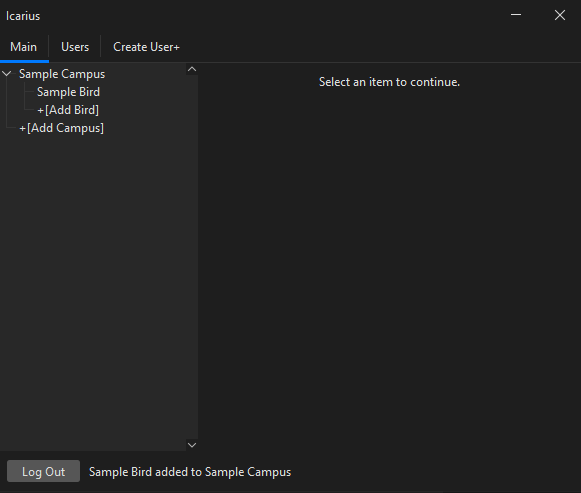
\includegraphics[width=0.6\textwidth]{MainTab/mainTab.PNG}
\end{figure}

The \textbf{Main tab} is where the user can add, edit and remove campuses, and within each campus the user can add, edit and remove birds. The main areas of the \textbf{Main tab} are listed below and are described in the following pages:
\begin{itemize}
    \item View Campus
    \item Add Bird
    \item View Bird
    \item Edit Bird
    \item Log Out
    \item Confirmation Message
\end{itemize}
The \textbf{Users tab} and \textbf{Create User+ tab} can be accessed by clicking on the respective tab.

\subsubsection{Adding a new bird to a campus}
In order to add a new bird to a campus, the user must:
\begin{enumerate}
    \item Click on \textbf{+[Add Bird]} located underneath the selected campus. \textit{This will reveal the \textbf{Bird Name} field}
    \begin{figure}[H]
        \centering
        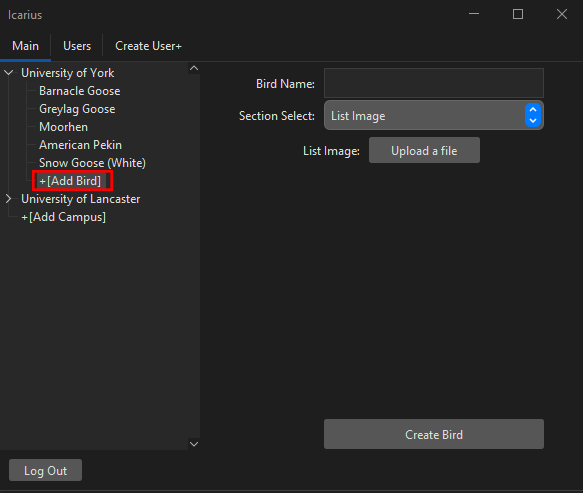
\includegraphics[width=0.6\textwidth]{MainTab/AddBird/addBird.PNG}
    \end{figure}
    
    \item Enter the name of the bird in the \textbf{Bird Name} field
    \begin{figure}[H]
        \centering
        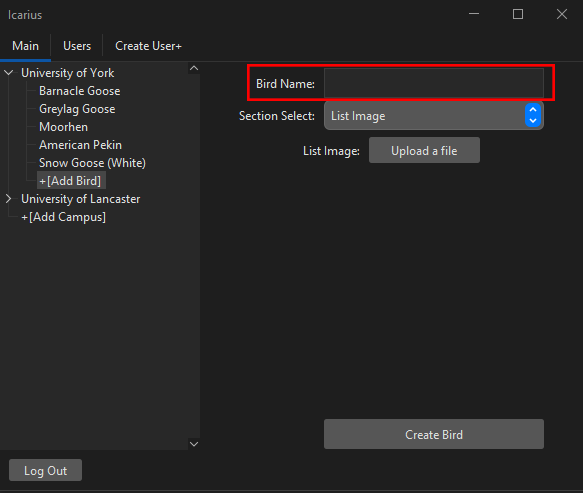
\includegraphics[width=0.6\textwidth]{MainTab/AddBird/addBirdName.PNG}
    \end{figure}

    \item Click the \textbf{Section Select} drop-down list to view each attribute of the bird
    \begin{figure}[H]
        \centering
        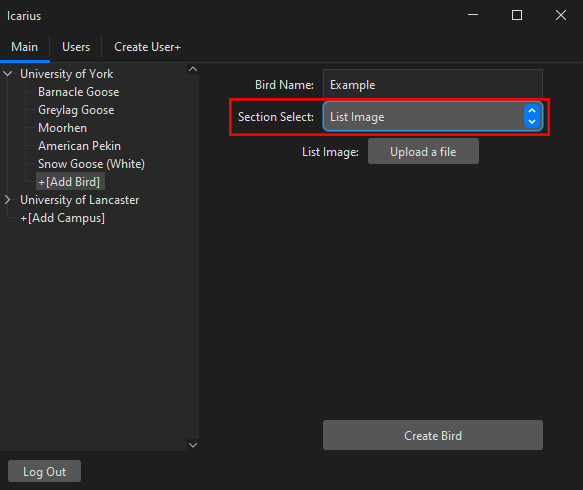
\includegraphics[width=0.6\textwidth]{MainTab/AddBird/addBirdSelect.PNG}
        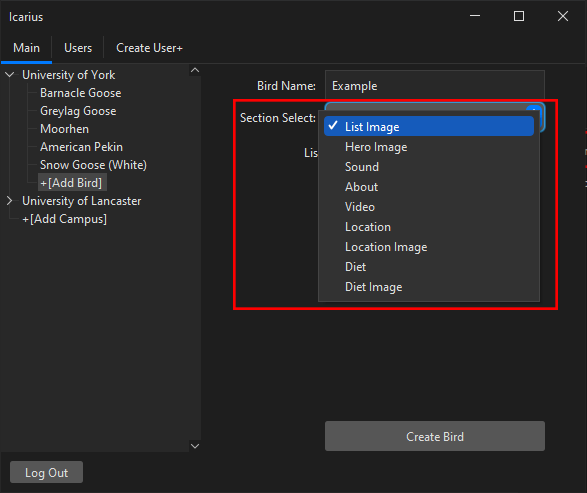
\includegraphics[width=0.6\textwidth]{MainTab/AddBird/addBirdDropdown.PNG}
    \end{figure}
    The attributes of a bird are as follows:
    \begin{itemize}
        \item \textbf{List Image:} The image of the bird as it appears in the bird list in FaunaFinder
        \item \textbf{Hero Image:} The image of the bird once clicked on in FaunaFinder
        \item \textbf{Sound:} The audio soundbite of the bird
        \item \textbf{About:} The information about the bird
        \item \textbf{Video:} The video footage of the bird
        \item \textbf{Location:} The location of the bird
        \item \textbf{Location Image:} The image of the location of the bird
        \item \textbf{Diet:} The information about the diet of the bird
        \item \textbf{Diet Image:} The image of the diet of the bird
    \end{itemize}
    
    \item Click on each section to fill in each attribute of the bird. \textit{Each attribute must be complete before the creation of the bird can occur}
    \begin{itemize}
        \item \textbf{List Image, Hero Image, Location Image and Diet Image:}
        An image can be uploaded for the attributes that require it by clicking on \textbf{Upload a file}. \textit{This will display the image underneath to confirm the correct image has been uploaded}
        \begin{figure}[H]
            \centering
            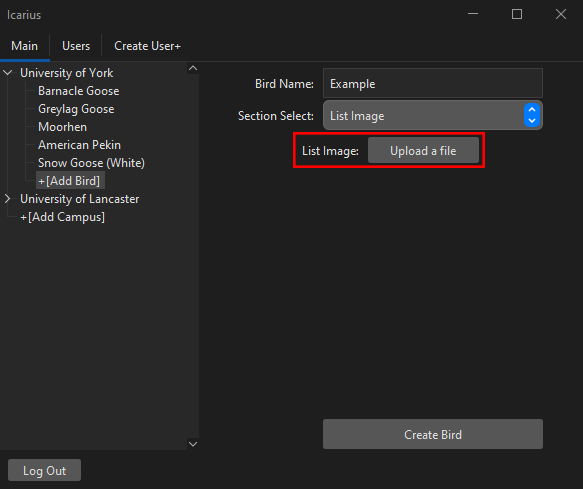
\includegraphics[width=0.6\textwidth]{MainTab/AddBird/addBirdImage.PNG}
            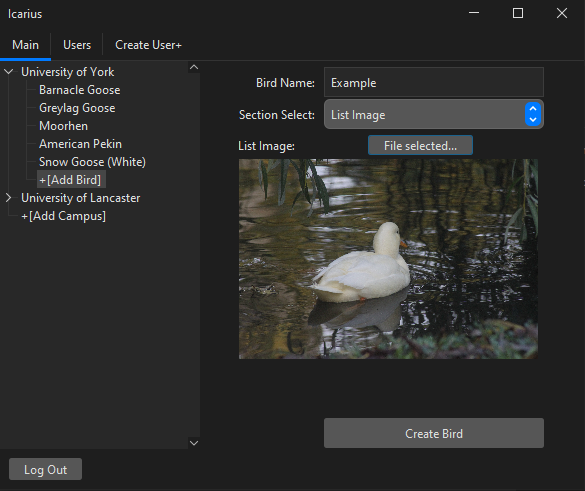
\includegraphics[width=0.6\textwidth]{MainTab/AddBird/addBirdImageSelected.PNG}
        \end{figure}
        
        \item \textbf{About, Location and Diet:}
        Information can be input for the attributes that require it by typing in the text area
        \begin{figure}[H]
            \centering
            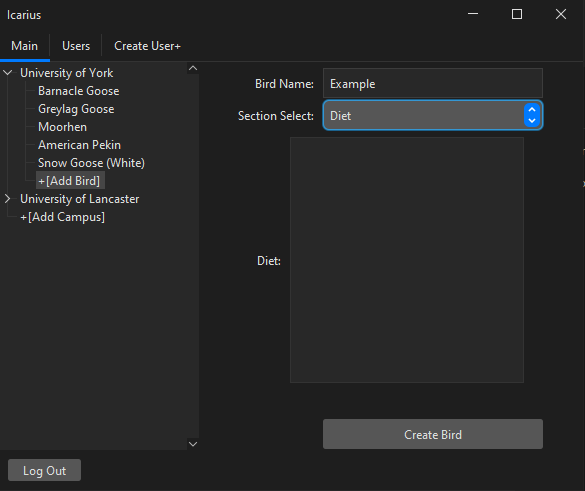
\includegraphics[width=0.6\textwidth]{MainTab/AddBird/addBirdText.PNG}
        \end{figure}

        \item \textbf{Sound:}
        An audio file can be uploaded by clicking on clicking on \textbf{Upload a file}. The audio can be sampled by clicking on \textbf{Play audio}
        \begin{figure}[H]
            \centering
            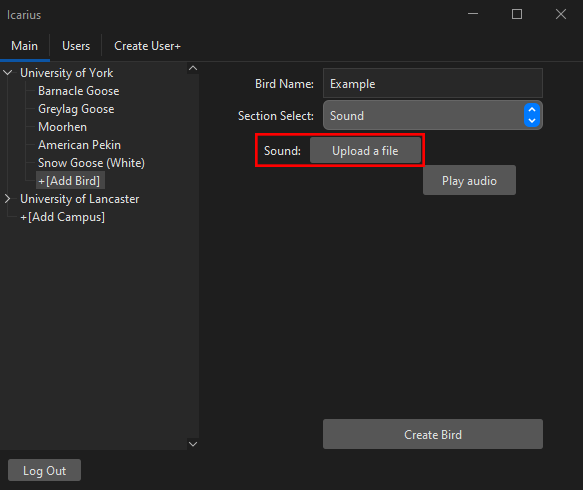
\includegraphics[width=0.6\textwidth]{MainTab/AddBird/addBirdAudio.PNG}
            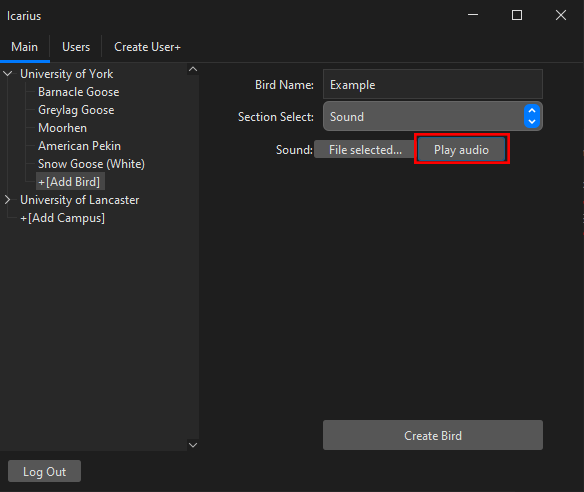
\includegraphics[width=0.6\textwidth]{MainTab/AddBird/addBirdAudioSelected.PNG}
        \end{figure}

        \item \textbf{Video:}
        A video file can be uploaded by clicking on clicking on \textbf{Upload a file}. A thumbnail preview of the video will be displayed below
        \begin{figure}[H]
            \centering
            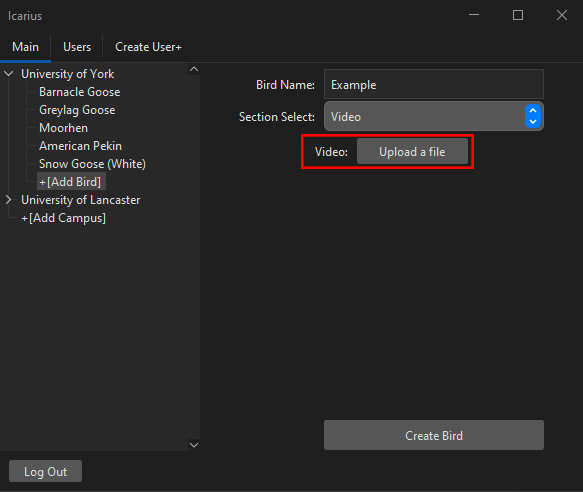
\includegraphics[width=0.6\textwidth]{MainTab/AddBird/addBirdVideo.PNG}
            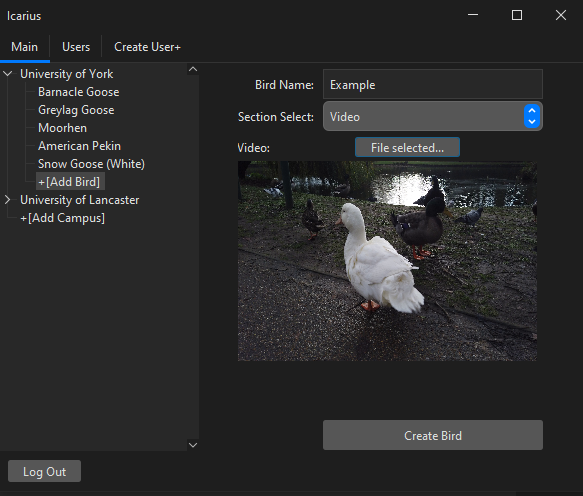
\includegraphics[width=0.6\textwidth]{MainTab/AddBird/addBirdVideoSelected.PNG}
        \end{figure}
    \end{itemize}
    
    \item Click the \textbf{Create Bird} button. \textit{This will add the bird to the database and display a confirmation button alongside the \textbf{Log out} button}
    \begin{figure}[H]
        \centering
        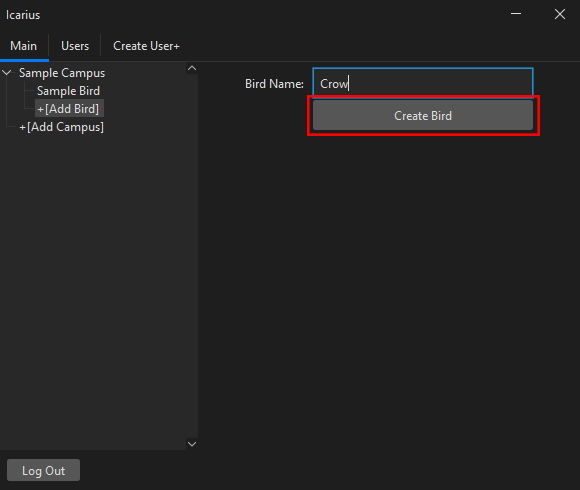
\includegraphics[width=0.6\textwidth]{MainTab/AddBird/addBirdCreate.PNG}
        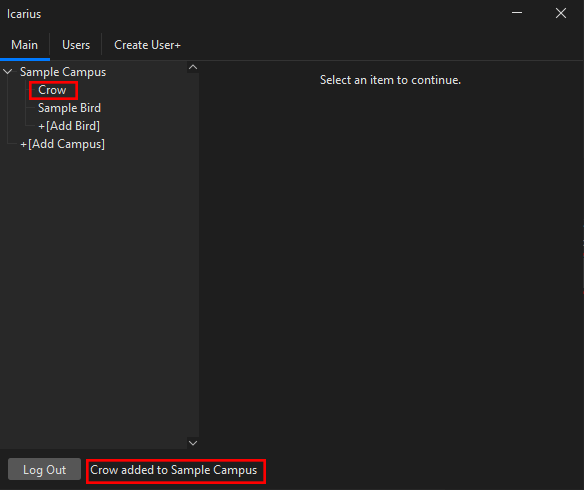
\includegraphics[width=0.6\textwidth]{MainTab/AddBird/addBirdCreated.PNG}
    \end{figure}
\end{enumerate}

\subsubsection{Editing an existing bird}
In order to edit an existing bird the user must:
\begin{enumerate}
    \item Click on an existing bird underneath the selected campus. \textit{This will reveal the details of that bird}
    \begin{figure}[H]
        \centering
        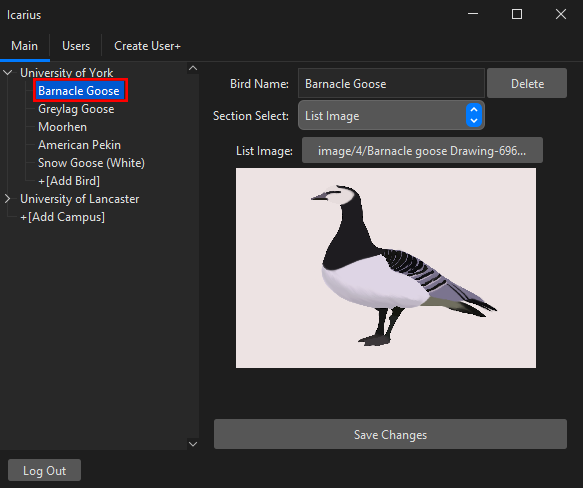
\includegraphics[width=0.6\textwidth]{MainTab/EditBird/editBirdView.PNG}
    \end{figure}

    \item From here, each of the attributes of the bird can be edited by selecting them from the \textbf{Section Select} drop-down list
    \begin{figure}[H]
        \centering
        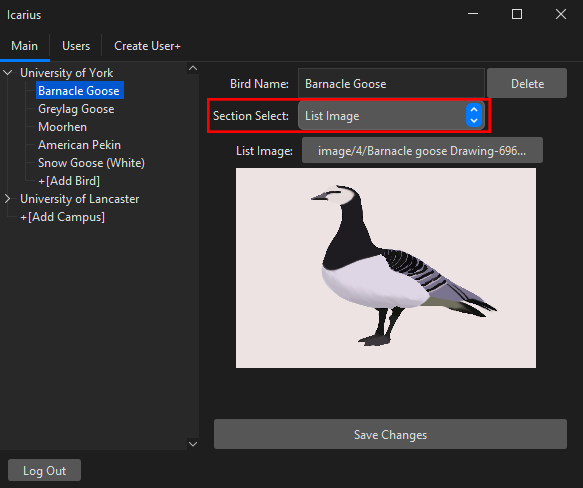
\includegraphics[width=0.6\textwidth]{MainTab/EditBird/editBirdSection.PNG}
    \end{figure}

    \item Clicking the \textbf{Save Changes} button will save the edits made to the bird to the database, whilst clicking the \textbf{Cancel} button cancels those edits made. The \textbf{Delete} button can be clicked to remove the bird from the database. \textit{Choosing \textbf{Save Changes} or \textbf{Delete} displays a confirmation button alongside the \textbf{Log out} button}

    \textbf{Save Changes:}
    \begin{figure}[H]
        \centering
        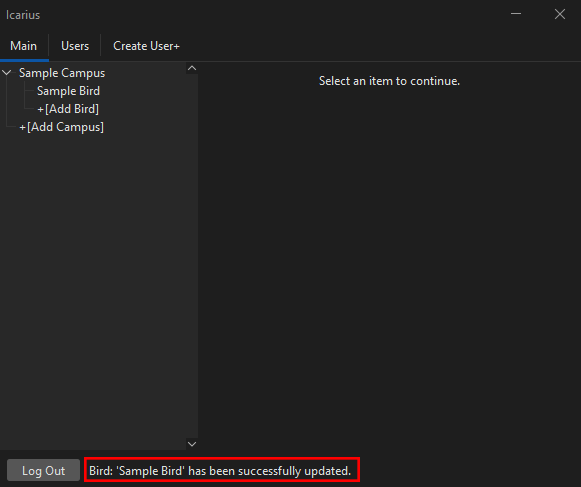
\includegraphics[width=0.6\textwidth]{MainTab/EditBird/saveChanges.PNG}
    \end{figure}

    \textbf{Delete:}
    \begin{figure}[H]
        \centering
        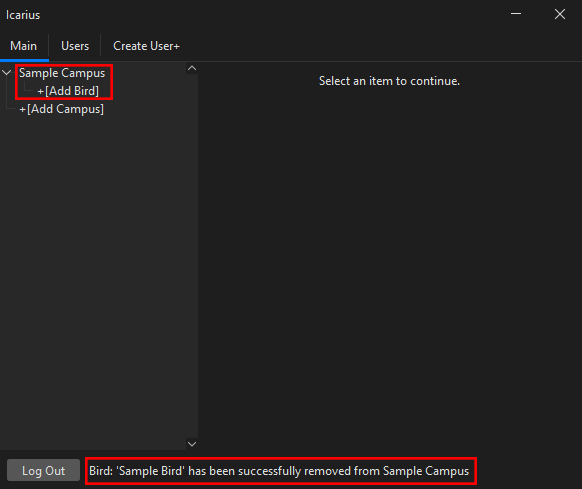
\includegraphics[width=0.6\textwidth]{MainTab/EditBird/deleteBird.PNG}
    \end{figure}
    

    
\end{enumerate}
